% Created 2017-12-21 Thu 11:45
\documentclass[12pt,a4paper,titlepage]{article}
\usepackage[utf8]{inputenc}
\usepackage[T1]{fontenc}
\usepackage{fixltx2e}
\usepackage{graphicx}
\usepackage{longtable}
\usepackage{float}
\usepackage{wrapfig}
\usepackage{rotating}
\usepackage[normalem]{ulem}
\usepackage{amsmath}
\usepackage{textcomp}
\usepackage{marvosym}
\usepackage{wasysym}
\usepackage{amssymb}
\usepackage{hyperref}
\tolerance=1000
\usepackage{microtype}
\usepackage[backend=biber, style=authoryear, natbib=true]{biblatex}
\addbibresource{ref.bib}
\usepackage{hyperref}
\usepackage[danish, english]{babel}
\usepackage{abstract}
\usepackage{algorithm}
\usepackage{algpseudocode}
\usepackage[a4paper]{geometry}
\usepackage{minted}
\usepackage{graphicx}
\usepackage{multicol}
\usepackage{subfig}
\setcounter{secnumdepth}{1}
\author{Brian Alberg}
\date{\today}
\title{}
\hypersetup{
  pdfkeywords={},
  pdfsubject={},
  pdfcreator={Emacs 25.3.1 (Org mode 8.2.10)}}
\begin{document}

\begin{titlepage}
        \begin{center}
        
\includegraphics[scale=0.3]{sdu_logos.pdf}~\\[6.0em]
        %\textsc{\large{University of\\[0.4em] Southern Denmark}} \\[6.0em]
        \textsc{\large{DM842}} \\[0.2em]
        \textsc{\large{Computer Game Programming}}\\[1.5em]
        \textsc{\large{Mandatory Project}}\\[1.5em]
        %a\rule{12cm}{0.5pt} \\[1.0em]
        { \huge \textbf{Ninja Castle}\\[1.5em] }
        %\rule{12cm}{0.5pt} \\[1.0em]
        \textsc{\large{Computer Science}} \\[6.0em]
        
        \large{Brian Alberg}\\[0.5em]
      \normalsize{brped13@student.sdu.dk}\\[1.5cm]
      
      \vfill

        {\large \today}\\[2em]
        \end{center}
        \newpage
\end{titlepage}

\section{Introduction}
\label{sec-1}
This report will document the 3D computer game Ninja Castle, which was
completed as a project for the Computer Game Programming course in the fall
of 2017, offered by the University of Southern Denmark.

The game is developed as a 3D-platform game with a 3rd person view, and takes
place in a castle-like arena, with 2 ninjas. One of the ninjas are controlled
by the player, and the other by an AI. The objective of the game is developed
based on the children's game \emph{King of the Hill}, where the objective is to
control a certain point or area, by keeping the other players away.

In Ninja Castle, this area is a platform located in the center of the arena,
connected to the rest of the castle by bridges, and surrounded by at moat.

The two players will start in each end of the castle, and the objective is to
control the center platform for the longest amount of time. This can be
archived by pushing the other player off the platform. If a player ends up in
the moat, he/she will respawn after 3 seconds. Points accumulate for each
second a player is on the center platform, and the player who first reach 500
points, will win the match, and the game will restart.

The process of the development will be documented in the \emph{Design and
Implementation} section, and screenshots will be attached to the end of the
report.

\section{Design and Implementation}
\label{sec-2}
\subsection*{Overall Structure}
\label{sec-2-1}
Ninja Castle was developed in C++ using as few dependencies as possible,
OpenGL being the most important one. It was planned to use \emph{modern} OpenGL
for the higher control of shading and other interesting topics, but because
of time constraints the end result is a mix of \emph{modern} and \emph{legacy} OpenGL.

Furthermore a few extension libraries was used to simplify certain OpenGL
related tasks.

\begin{itemize}
\item The \emph{GLUT} toolkit was used for system-related activities, such as creation
of the window application, listening for keyboard-input, etc.
\item The \emph{Glew} extension were used to handle modern OpenGL API functions at run-time.
\item The \emph{GLM} library were used to simplify certain vector-related tasks with
respect to OpenGL.
\end{itemize}

A lot of time was put into a decent overall structure of the project, as it
contains many diffirent elements which should be able to communicate
appropriately, however a few things were hard-coded where needed to save
time. Below is a short summary of the overall structure.

\begin{itemize}
\item The Collision class in \emph{core.cpp} contains methods for collision
and physics related functionality. The collision class will get feedback
from the characters about their current position and rotation.

\item The Character class contains functionality related to initialization,
drawing and movement of a character and utilizes some functionality of
the Collision class e.g. checking for collisions with the other character
and walls.

\item The Player and AI classes inherits functionality of the Character
class, with the AI class extending with the code for the AI.

\item The Map class contains functionality to initialize the map from an .obj-file,
and draw the map.

\item The Material class contains functionality to load/read material files, and
store this data for usage on objects.

\item The \emph{main.cpp} file contains everything related to the GLUT toolkit, such
as keyboard listeners. It also sets certain OpenGL parameters, calls the
initialization procedures of the different classes, and calls the draw
procedures of the different classes, where appropriate. Furthermore, the
score of the individual characters, while calculated in the character class,
is handled here.
\end{itemize}

\subsection*{Graphics}
\label{sec-2-2}

\begin{figure}
      \centering
      \begin{subfigure}
            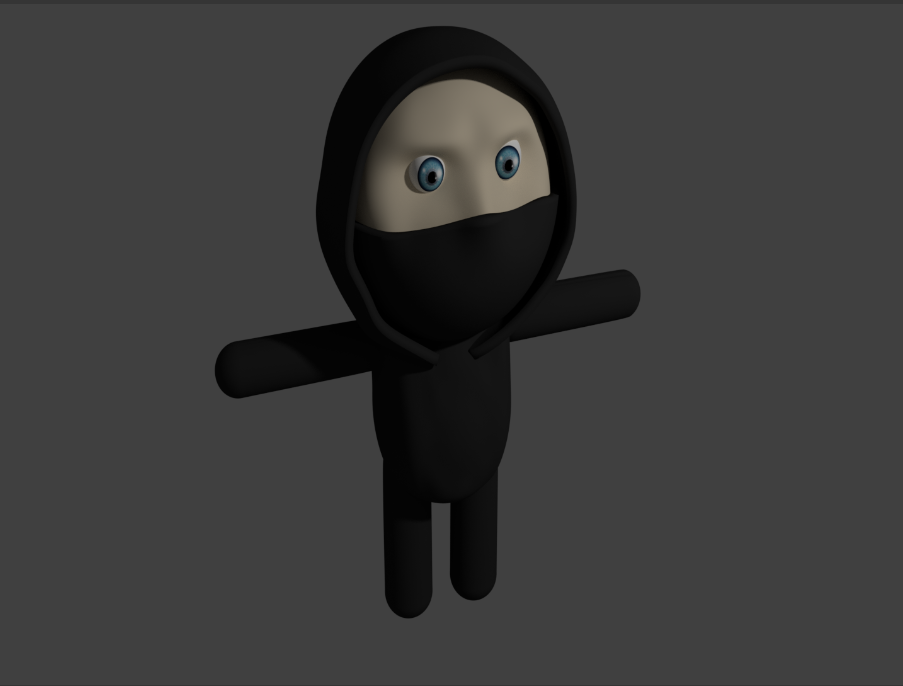
\includegraphics[width=0.4\textwidth]{char1.png}
      \end{subfigure} 
      \begin{subfigure}
            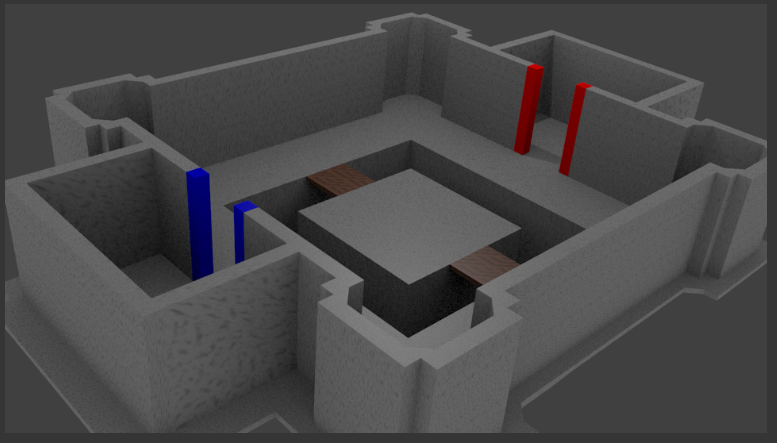
\includegraphics[width=0.53\textwidth]{map1.png}
      \end{subfigure} 
      \caption{Early 3D models of ninja character and castle map in Blender}
      \label{fig:blender}
\end{figure}

The graphics for Ninja Castle was the most time consuming part of the
project, as it included going through much of the OpenGL documentation, to
archive the desired result. Two 3D models were made using the Open Source
3D suite \emph{Blender}, a ninja-like character model, and a model for the map,
as shown in figure \ref{fig:blender}. The eye/pupil-texture on the Ninja's
eyeballs was dropped at a later stage in the project, since it was the only
actual texture, and other parts of the project needed more attention.

\begin{figure}
      \begin{minted}{text}
mtllib [material file name]
usemtl wood
v 0.123 0.234 0.345
...
vt 0.500 1
...
vn 0.707 0.000 0.707
...
f 1 2 3
...
      \end{minted}
      \caption{Structure of a .obj file.}
      \label{fig:objfile}
\end{figure}

To use these figures with OpenGL, they were exported into Wavefront \emph{.obj} files,
which is a plaintext format able to store information about a 3D model, such
as vector and face information, corresponding material, texture (UV)
coordinates and vector normals. Each line starting with a \emph{v} is a
definition of a vector, and is followed by its 3 scalars/coordinates. The
same applies to the normal vectors, except these are defined by \emph{vn}. Faces
are defined by a line starting with \emph{f}, but are instead pointing to 3
previously defined vectors, by 3 indices. \emph{mtlib} and \emph{usemtl} defines a 
material (.mtl) file, and a specific material from that file, respectively.
An example of the formatting is shown in figure \ref{fig:objfile}.

The .mtl files are similarly formatted, but instead contain RBG values
similar to what is used by OpenGL's \texttt{glMaterial} function, hence each a line
for ambient, specular and diffuse light, for each material.

All of these exported files are parsed using parsers developed specifically
for this project, and the values are put into buffers. After this, the values
are \emph{pushed}, or \emph{uploaded} to the memory attached to the GPU. This is done by creating
\emph{Vertex Buffer Objects} or \emph{vbo}'s, more specifically a \emph{vbo} for each of the
following: vectors, colors and normals.  These \emph{vbo}'s are then attached to a
\emph{Vertex Array Object}, with a definition of what kind of data the \emph{vbo}
contains. After this step, all data is on the GPU memory and can be refered
to by refering to the \emph{vao}, which points to several \emph{vbo}'s containing the
actual data.

The drawing step is now as simple as refering to the \emph{vao}, and make a call
to \texttt{glDrawArrays} for each 3D object.

\subsection*{Artificial Intelligence}
\label{sec-2-3}
A simple AI was developed for the AI-controlled character. The objective of the
AI is to win the game by moving into the center platform in a heuristic seek-like
manner. A great improvement would have been to implement a heuristic shortest
path algorithm, and this was actually planned, but was dropped because of
time constraints. The AI will try to find the center of the map by using a
\emph{target} point i.e. the center point of the map, which is simply and $x$,$y$
value. Furthermore, 4 rays are defined, each as a $x$,$y$ value, as follows:

\begin{align*}
front &= \{x + \sin(angle), y + \cos(angle)\}\\
left &= \{x + \sin(angle-90),  y + \cos(angle-90)\}\\
right &= \{x + \sin(angle+90), y + \cos(angle+90)\}\\
back &= \{x + \sin(angle-180), y + \cos(angle-180)\}
\end{align*}

$x$, $y$ and $angle$ being the $xy$-position and angle of the AI character,
respectively. For each of these rays, a distance is calculated, using the
euclidean distance, from the position of the ray on the map, to the \emph{target}
point. A final distance is defined as being the distance from the position of
the AI itself, to the target point.

The AI will now move around much like a robot vacuum cleaner, trying to
minimize the distance from the AI character, and the center point. However,
if the front ray detects a wall in front of it, or the moat, it will stop
moving, and turn. The direction in which the AI will be turning, can be
defined as:

\begin{align*}
\delta = \min(d(left, target),\, d(right, target))
\end{align*}

where $d(p,q)$ is the euclidean distance between $p$ and $q$, and where if
$\delta = d(left, target)$ means a turn to the left.

This is similar to how the AI determines the direction in which it should go
if not obstacles are in its way.

To make the AI a bit more interesting, a \emph{chase} state was added. If the
distance between characters of the AI and the player reaches below a certain
threshold, the
AI will change its \emph{target} to the position of the players' character instead. In
practice this means that if the AI and the player is not near each other, the
AI will seek towards the center platform, and stay there. However, if they a near each
other, like in the case where both the AI and the player are on the center
platform, the AI will change its objective, and try to push the player off
the platform. If the player get further away from the AI than the given
threshold, the AI will change its \emph{target} to the point on the center
platform once again.

\subsection*{Collision Detection}
\label{sec-2-4}
\subsubsection*{Wall Collision}
\label{sec-2-4-1}
Collision detected was implemented in multiple parts of the project. The
most important being the collision with the walls of the level, since the
characters should not be able to walk through the walls. To prevent having
to check for collisions between the walls in all 3 dimensions, i.e. by
comparing coordinates of vertices, a more simple, yet suitable approach was
discovered.

On initialization the map.obj file is parsed to find the vectors that
correspond to the floor of the map. As mentioned earlier, a face is made up
of three vectors, to make a triangle. Hence, the floor is also made up of
triangles, which is made up of vectors.

The problem of detecting whether the character is within the boundaries of the
map, is now simplified to detecting whether the $xy$-position of the
character is within any of several triangles. Hence, the Barycentric coordinates
is computed for the position of the character (or actually a point slightly
in front of the character) with respect to each triangle that make up the
floor. By defining $p$ to be the position of the character, and $p1$, $p2$
and $p3$ to be the three points, or three 2-dimensional vectors, that defines
a triangle, the Barycentric coordinates can be computed as

\begin{align*}
  \alpha &= \frac{(p2_y - p3_y) * (p_x - p3_x) + (p3_x - p2_x) * (p_y -
  p3_y)}{(p2_y - p3_y) * (p1_x - p3_x) + (p3_x - p2_x) * (p1_y - p3_y)}\\
  \beta &= \frac{(p3_y - p1_y) * (p_x - p3_x) * (p_y - p3_y)}{(p2_y -
  p3_y)*(p1_x-p3_x) + (p3_x - p2_x) * (p1_y - p3_y)}\\
  \gamma &= 1 - \alpha - \beta
\end{align*}

The values of $\alpha$, $\beta$ and $\gamma$ can now be checked. If
$\alpha,\beta,\gamma > 0$ it means the center point of the
character is inside the triangle that defines a part of the floor. Hence,
there's no collision with a wall. Otherwise, there's a collision.

When a character moves, a ray of a certain length is cast in front of the
character with respect to the facing angle of the character. This ray is used
to check if there is a obstacle ahead. However, since the floor is used to
check for collision, by the above definition, the moat is an obstacle too. To
avoid this, the restriction of character movement is only applied when
outside of the center area. If the character is inside the square that makes up the moat and
the center platform, and a \emph{collision} happens in this area, the characters'
movement is not restricted, and hence this makes it possible for the
character to fall down the moat, even though it actually triggers a
collision.

Furthermore, if the character is inside the center area, and there's no floor
below the character, it means the character is on the moat. In this case the
character falls down, which will be described in the Physics part, and then
yet another collision happens. When a characters' $z$ (or in some games $y$)
position reaches below a certain threshold (below the floor), the character
enters a state of paralysis, where all movement is disabled, and then the
characters' state change to \emph{dead}. At the same time a timer is startet, to
determine when the character should respawn.

\subsubsection*{Character Collision}
\label{sec-2-4-2}
Collision between the two characters is checker in a trivial way, by using the
Euclidean distance between the two characters. If the two characters are closer
than a certain threshold, a collision between the characters are detected.

But detecting by the distance between two points $p$ and $q$, $d(p,q) =
d(p,q)$ in all cases. Hence, a collision between the two players, will always
result in a collision for both players. Because of this, the way they collide
was slightly tuned because of this. Instead of using the distance between the
two characters, a ray was cast in front of each characters. By using the
front ray instead of the center point of the character to calculate a
distance to the enemy character, it means that a character is only able to
attack, or push, the enemy by facing him. Hence, it is potentially possible
to hit an enemy, without getting hit yourself, e.g. by walking into him from
the side, or behind.

\subsubsection*{Center Mechanics}
\label{sec-2-4-3}
As mentioned earlier if the character is inside the center area, and there's
no floor
below the character, it means the character is on the moat. In this case the
character falls down, which will be described in the Physics part. When the
character reaches below a certain threshold on the axis that is the normal
vector of the floor plane,a collision happen. This collision will make the
character enter a state of paralysis, where all movement is disabled, and then the
characters' state change to \emph{dead}. At the same time a timer is startet, to
determine when the character should respawn.

Another mechanic of the center of the map, is used to calculate the points
given to each character. The Euclidean distance was calculated between each
character and the center of the map. If the distance is below a certain
threshold, a timer is started, which will give the character points, based on
the number of seconds spend on the center platform. If the player gets above
the threshold, meaning too far away from the center platform, the timer will
stop. A slight tweak to this mechanic would clearly be to use a better
distance measure than the Euclidean distance, as the center platform clearly
isn't circular.

\subsection*{Physics}
\label{sec-2-5}
Trivial physics was developed for parts of the project, and is what is used
for character jump, and when a character is detected to be in the moat, as
defined above. In both these cases, a velocity variable is increased, and
from that, and a gravity constant, a new position of the character is
calculated, and the velocity variable is decreased. To take time into account,
the calculation of the new position is restricted to only be calculated and
adjusted 50 times per second.

Another part of the game was not as
trivial as it probably should have been. As already mentioned, character
collision happens when the distance between the front ray of a character, and
the center point of the enemy character gets below a certain threshold. The
idea was, that when this collision was detected, the enemy character should be
launched up in the air, and away from the attacking character. 

The way it was to be implemented was to compute a velocity vector based on
the angle of the attacking character. Unfortunately this was not as trivial
as anticipated, and was not implemented correctly before delivery. In some
cases it will work, but in others the enemy character will not be launched
away from the attacking charachter, but just slightly up in the air.


\section{Conclusion}
\label{sec-3}
The project was a lot of fun and very giving because of the given freedom.
While more time was probably spent on the project than what should have, all
planned parts was implemented in some way or another. As stated a moment ago,
the biggest shortcoming of the project, was most likely the lack of better
physics, and if more time was given, that would be the first thing to improve
on.

On a further note, an implementation using \emph{modern} OpenGL would have been
beneficial to get full control of the shading. Textures was not implemented
either, but for the simplicity of the project, it did not feel important
enough (basically the only texture on the initial 3D models was the pupils on
the eyes of the ninja model). To improve even further, animation of the
characters would have given alot to the project, but it was discovered early
on that animation, while rather trivial with regards to implementation, is a tedious
task when it comes to making the 3D models.

The AI part was especially interesting, and as
already stated, more work could have been put into making a more clever AI.
When that is said, the AI, while not being as smart as a real player,
actually fulfill its purpose by challenging the player in reaching his/hers
objective. That is, if the player do not take advantage of the minor flaws in
the game.


\newpage
\section{Screenshots}
\label{sec-4}
\begin{figure}[h]
      \centering
      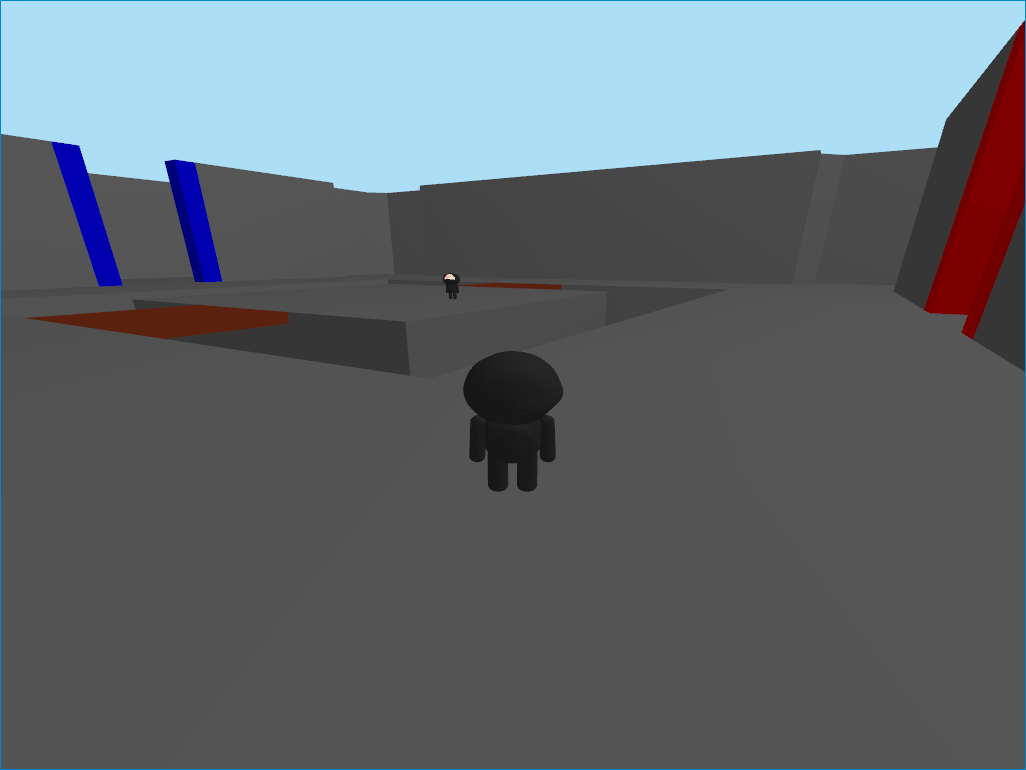
\includegraphics[width=\textwidth]{screen1.png}
      \caption{Final game. AI have taken control of the center platform}
\end{figure}

\begin{figure}[h]
      \centering
      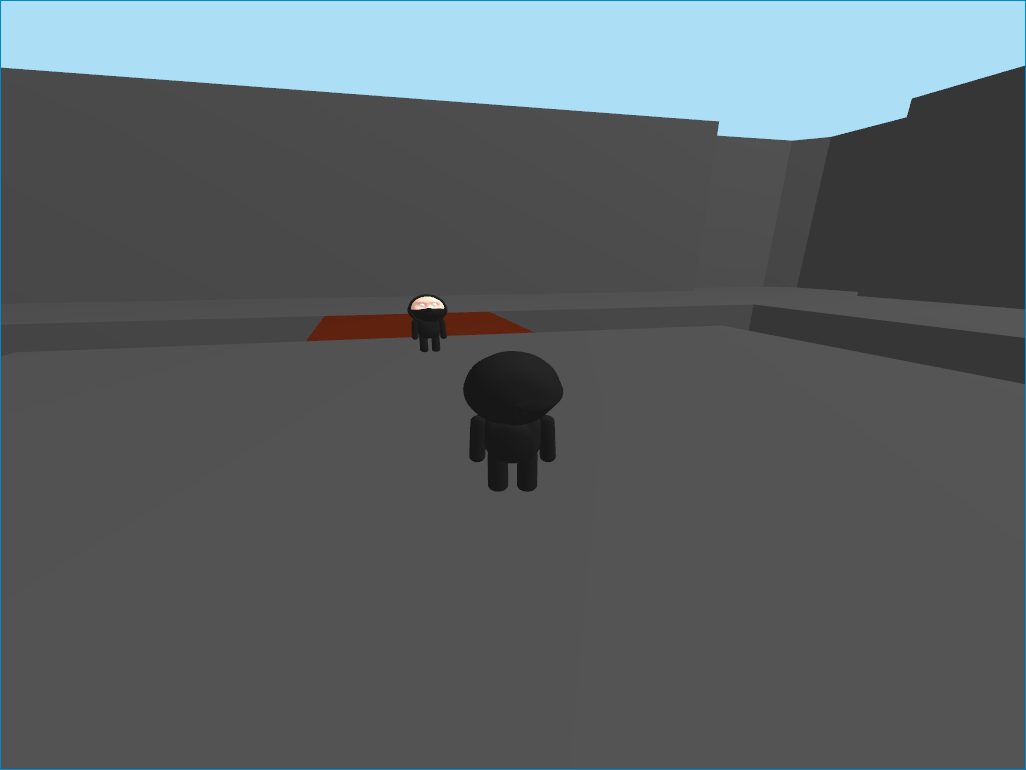
\includegraphics[width=\textwidth]{screen2.png}
      \caption{Final game. AI-controlled character approaching}
\end{figure}

\begin{figure}[h]
      \centering
      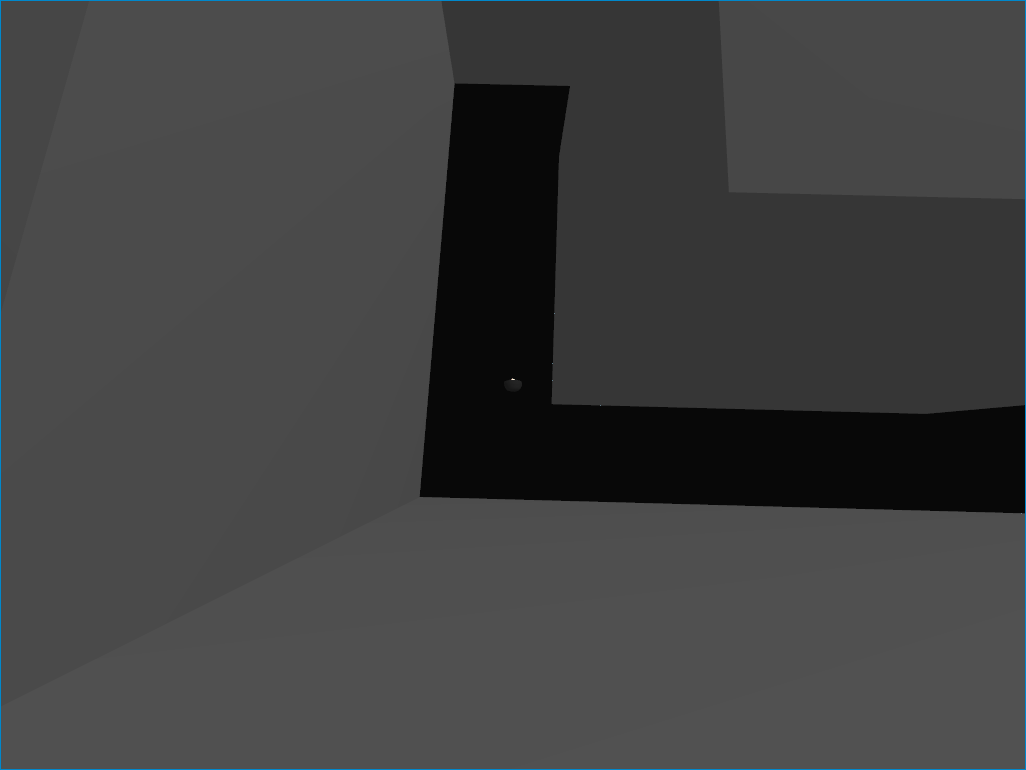
\includegraphics[width=\textwidth]{screen3.png}
      \caption{Final game. Player died}
\end{figure}

\begin{figure}[h]
      \centering
      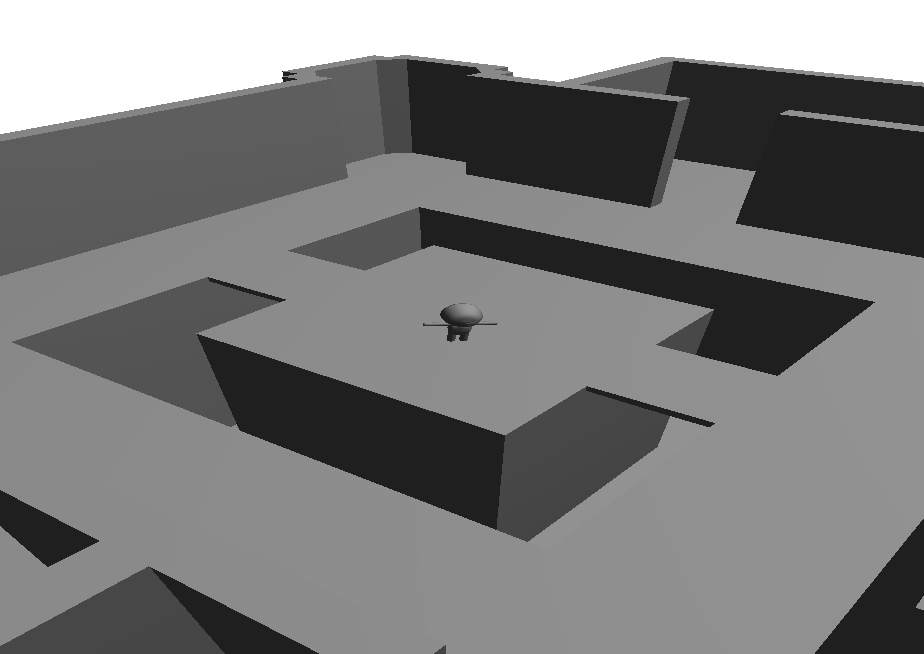
\includegraphics[width=\textwidth]{screen0.png}
      \caption{Early stage of the game, testing the .obj parsers}
\end{figure}

\begin{figure}[h]
      \centering
      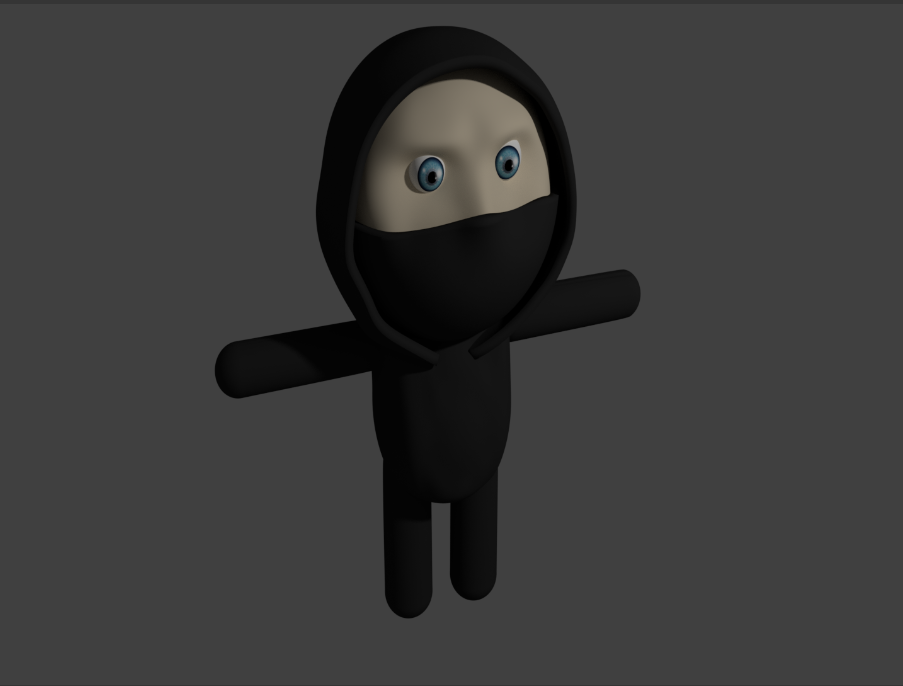
\includegraphics[width=\textwidth]{char1.png}
      \caption{3D model of the ninja, before the eye texture was removed, and
      arms put down}
\end{figure}

\begin{figure}[h]
      \centering
      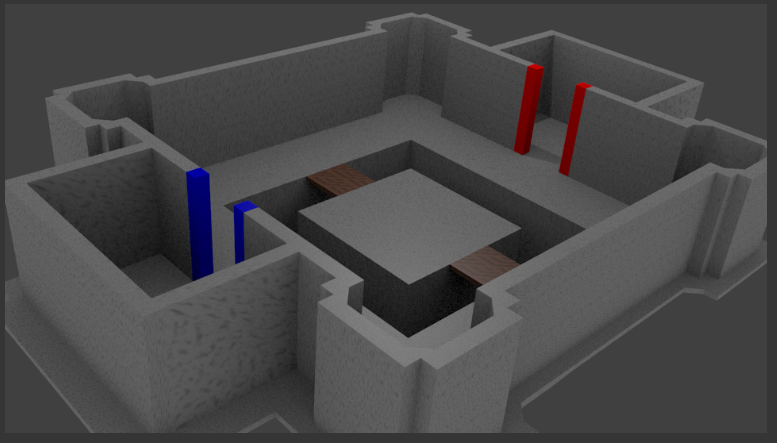
\includegraphics[width=\textwidth]{map1.png}
      \caption{3D model of the castle map}
\end{figure}
% Emacs 25.3.1 (Org mode 8.2.10)
\end{document}
